\documentclass{article}[11pt]
\usepackage[portrait, margin=1in]{geometry}
\usepackage{graphicx} 
\graphicspath{{/Users/danpost/housing_project/output/prospectus/graphics}}
\usepackage{amsmath}
\usepackage{hyperref}
\usepackage{booktabs}
\usepackage{array}
\usepackage{comment}
\usepackage[authordate, backend=bibtex, natbib]{biblatex-chicago}
\addbibresource{prospectus_bib.bib}

\begin{document}

\title{Politics, Credit Access, and the Dynamics of Housing Markets} 
\author{Daniel Posthumus}

\maketitle

\section{Introduction}
Why, as labor productivity, output, and aggregate demand have all increased, has the United States gotten \textit{worse} at building housing? This is a question whose answer we understand fairly well; burdensome regulation has made it more difficult to build. This is the core argument of the ``abundance agenda" (also referred to as ``supply-side progressivism"), which liberal commentators (most prominently Ezra Klein and Derek Thompson) have centered in their arguments over why Democrats lost the election in 2024 and how liberalism can redeem itself.\footnote{To be clear, the idea of supply side progressivism preceded the 2024 election and went hand-in-hand with the post-COVID development of Bidenomics. The agenda has two leading focuses: energy and housing. In this paper, I focus on the latter. For an introduction to the way the abundance agenda addresses energy, see \citep{cheap2022energy}. While the abundance agenda motivates the urgency of the puzzle I identify, I don't center it in this paper.} \citep{klein2021economic} \citep{kleinthompson}

With respect to housing, the abundance agenda highlights a basic misallocation problem: it is very hard to move to the most productive places in the United States of America. It's hard because housing is too expensive there: construction and supply in these places has not kept up with demand because burdensome regulation has choked off supply. \citep{glaeser2005} \citep{glaeser2005empirical} The economics of this are well-established; scholars have demonstrated that housing prices are higher because of land-use regulation, and they have demonstrated this has led to a misallocation of labor which has devastating effects on aggregate output. \citep{hsieh2019housing} In this framing, politics, not economics, has prevented the ``invisible hand" of the market from operating. In this version, \textit{housing markets are out of equilibrium}. Klein and Thompson have a simple solution: remove the bottleneck of politics, and markets will achieve equilibrium and prices will come down.

This argument is well-founded, although I think its literature neglects two areas: politics and credit access.\footnote{Again, my focus here is on the academic literature, not the work in popular media by bloggers/writers like Matt Yglesias, Noah Smith, Klein, and Thompson. However, many of the flaws in the literature are reflected in the work of these bloggers. The literature's lack of understanding of politics in developing regulations for example, can be reflected back as these bloggers' lack of awareness. To pick an easy example, a recent \href{https://www.slowboring.com/p/new-york-city-can-do-better-than}{article} by Yglesias' media company \textit{Slow Boring} touts a New York City mayoral candidate Zellnor Myrie for his pro-housing policies. \citep{zellnor} Myrie is, according to \href{https://poll.qu.edu/images/polling/nyc/nyc03052025_nytv24.pdf}{Quinnipac}, polling at 1\%. This gap--between Myrie's popularity among `thinking liberals' and his popularity with voters--is not seriously addressed in the piece and is part of a broader overlooking of popular politics among abundance thinkers.} First, housing policies are endogenous; they are, by definition, the result of political processes which are determined by constituents -- the composition of which is dependent on who can afford the housing in a community. Second, the literature does not adequately incorporate access to credit into models; in particular, we don't understand how interventions in credit markets affect housing markets when interacted with supply,\footnote{Demand models of housing have convincingly incorporated credit access.}

There are many ways to approach these challenges, and I am not close to formalizing a model and presenting results. What I do in this paper is first prove there is a puzzle that needs to be answered: \textbf{we don't have a complete model of housing market equilibrium or disequilibrium that effectively incorporates 1) politics, 2) credit access, and 3) dynamics}. This puzzle matters: housing policy is deeply broken in America, but to fix it people need to understand how to structure capital access, and the political processes which produce and result from the very housing regime that economists have thoroughly demonstrated is economically broken. 

In the second half of this paper, I explore some specific ways I can operationalize and understand this broad theme. One little-understood question that politicians and policymakers want an answer to are the effects of the Community Reinvestment Act (CRA). I briefly discuss previous work on the CRA, before proposing new research on its effects on housing markets through expansions (or contractions) in credit access. Another proposal is to harness the richness of zoning commission hearing data through the most novel Large Language Models (LLMs) methods to develop rich data on the political \textit{process} of regulation-making, something we simply don't have good data on but would be a good way of overcoming the endogeneity of housing policy. Finally, I conclude with the broad brush strokes of a historical project. We don't know have a good idea of what housing markets looked like before zoning; I propose an expansion on previous work using historical newspapers to develop a real estate listing-level dataset for the pre-zoning era. These ideas can be disparate (and threateningly unwieldy) at times and not all provide solutions to the puzzle I lay out; however, I believe that the ultimate goal of these ideas is to produce separate pieces of empirical evidence which can then be synthesized into a theoretical expansion in how we thinking about housing.

\section{Literature Review}

The research puzzle I identify lies at the intersection of diverse literatures; here,I focus on the broad strokes of 3 literatures. First, I establish that a large literature finds that exclusive and constrictive land use regulation exists in the United States and that this regime has harsh, negative economic effects through raising prices and 2nd- or 3rd-order effects such as labor misallocation and lower construction productivity. Some papers have addressed regulation's endogeneity, although this remains an unsolved challenge. Second, I demonstrate that some scholars have focused on the role of credit access in shaping housing markets. This literature is distinct and unconnected to empirical work on regulation and structural housing models, even though the very notion of credit access is deeply embedded in housing markets. Finally, some scholars have previously tried to build structural models of housing markets. I explain how these models are incomplete, given the established empirical importance of politics and credit access in housing.
		
	\subsection{Land Use Regulation}
In the early-mid 2000s, an influential series of articles appeared first establishing the existence of exclusionary zoning restrictions and demonstrating these restrictions were leading to increased housing prices. Although previous work was aware of this phenomenon and its effects, the mid 2000s wave of papers was critical in systematizing our understanding of regulation and its effects. Fischel (2004) provides a thorough economic historic review for \textit{why} exclusionary zoning policies exist. \citep{fischel2004economic} Fischel was prominent for developing a theory that homeowners became \textit{homevoters}, i.e., they would vote for their homes in local elections and at public hearings. Homeowners have a significant financial asset that can increase in value through the achievement of certain policies, so they will push hard for those policies. Fischel's theory is also that homeowners tend to be commuters; hence zoning's initial coinciding with the expansion of streetcar suburbs in the 1910s and 20s and its later expansion under suburbanization and urban renewal in the 1950s and 60s.\footnote{Fischel's approach may seem slightly dated to the reader in 2025; he argued that homeowners were worried about their homes \textit{losing} value, and that zoning was protection against that possibility through increases in density. Today, one might take for granted their homes in high-productivity areas with restrictive land regulations are perpetually gaining in value, such that when one buys a home one expects not just a steady investment, but significant appreciation over time. This distinction is not central to what I see as Fischel's main contribution, which is explaining the emergence of these regulations between 60-100 years ago, but I think it merits mention.} 

The basic fact of constrictive zoning regulations established, I turn to its effects. Pre-2005, Quigley and Rosenthal document a breadth of papers showing a significant positive association, though not causal relationship, between land use regulation and housing prices. \citep{quigley2005effects} Glaeser et al. built on this work to more thoroughly solve a puzzling phenomenon: the cost of building a house stagnated from 1970 to 2005, while housing prices increased astronomically. \citep{glaeser2005empirical} Their argument was that the literature had previously focused on demand-side explanations, while the truth lie on the supply side, which was constrained by restrictive zoning regulations. While Glaeser et al.'s empirics are largely descriptive, they spawned analysis of further effects of zoning regulation beyond the 1st-order price effects.\footnote{Glaeser et al.'s empirics focus on disproving alternative explanations for the divergence of housing prices and construction costs. They show that only about a quarter of this gap could be explained by increases in housing quality. Next, they show that high demand (measured by the ratio of price to construction costs) in the 1970s drove new construction in the following decade, whereas that basic relationship was reversed as soon as the 1990s. \textit{High prices no longer led to new construction}, suggesting the reason for those high prices was not high demand, but low supply which can't easily be expanded. They formalize some of these ideas into a model which I briefly discuss below.} 

Elevated housing prices have tremendous 2nd- and 3rd-order effects: if housing prices increase in a given area, fewer people can afford to live there. This may lead to spatial misallocation of workers if the most productive firms are located in places with stricter regulations and higher prices (prominently San Francisco, for example). Hsieh and Moretti find that if San Francisco, New York City, and San Jose reduced land use regulations to the level of the median city, their growth rate of aggregate output would be 36.3 percent higher -- resulting in a stunning 3.7\% increase in US GDP in 2009.\footnote{This finding and its magnitude serve as a key motivator for the abundance agenda, although notable critiques of the abundance agenda's focus on increasing the aggregate output of these high-productive metros wonder why the movement wouldn't focus on increasing productivity in less-productive areas. \citep{abundanceambiguity}}\footnote{More restrictive zoning policies have also been associated with a greater share of residents commuting and working in another community in California. \citep{durst2021land}}  \citep{hsieh2019housing} Another proposed effect of regulation is a weakening of construction productivity, specifically the growing gap between manufacturing traded good productivity and construction productivity in the United States. D'Amico et al. (2024) demonstrate that constrictive regulation has resulted in smaller construction firms and smaller construction projects, which accounts for a very large share of the gap between manufacturing and construction productivity. \citep{d2024has} \footnote{There are other exciting advances in this literature. Bartik et al. use Large Language Models (LLMS) to interpret statutes and create advanced non-survey-based data on zoning laws. \citep{bartik2024costs} Gabriel and Kung find regulations manifest in extreme development approval times, reducing housing production and productivity through a construction-level dataset. \citep{gabriel2024development} Glaeser and Ward find that restrictive regulations cause less construction and higher prices, unless you control for contemporary neighborhood characteristics such as demographics and density. \citep{glaeser2009causes} Of course, if we accept that regulations cause lower density, then its lack of significance upon controlling for density in no way means it doesn't have an upward effect on prices.} 

\begin{comment}
The empirical analyses I discuss above were largely limited by the lack of a comprehensive dataset on zoning restrictions and housing policy in general; since the publication of his 2005 paper with co-authors, Gyourko has compiled two waves of a nation-wide survey on local regulatory environments, one in 2007 and the other in 2021. \citep{gyourko2008new} \citep{gyourko2021local} To summarize, Gyourko and his co-authors sought data on 1) general characteristics of the regulatory process, 2) specifics of the local residential land use regulation, 3) outcomes of the regulatory process, 4) state-level analyses of land use policy actions, and 5) measures related to environmental and open space-related ballot initiatives (the latter two categories of variables weren't directly part of the survey but were supplemented by the authors' own analysis. Another prominent survey, the Terner California Residential Land Use Survey, focuses on California--although it has the drawback of only having one wave of data, from 2017-2018. \citep{mawhorter2018terner} In general, data has lagged behind formal modeling as it relates to housing supply exclusionary zoning -- \textit{particularly along the dimension of time}. \citep{gyourko2015regulation} Nonetheless, extensive progress has been made in data for urban and regional economics the last 10 years. \citep{newdata} With regard to historical data, much of this work has been made by digitizing paper maps (to obtain census tract- or neighborhood-level boundaries used to geographically categorize households, that we could pull from historical Census records, the complete microdata of which is released 72 years after it was fielded). These historical maps and linked census data have allowed researchers to track historical neighborhood formation and segregation within cities.}
\end{comment}

	\subsection{Credit Access and Housing Markets}
Credit access matters in housing markets; this is because access to credit is necessary for the vast majority of homeowners to purchase their homes, credit in the form of mortgage loans. Thus, we can't accurately model housing demand without incorporating credit. I don't dwell on this literature because I'm not arguing it's inadequate; instead, I argue below that the literature on housing structural models don't adequately incorporate credit access. Thus, here I simply establish that credit access matters.

There is a wellspring of evidence showing credit access matters. Dettling and Kearney show that the drastic expansion of home ownership rates post-WWII was the result of the creation of the modern US mortgage system. \citep{dettling2025did} Specifically, they isolated variation in the \textit{supply} of loan issuance to show that mortgage insurance programs greatly expanded home ownership and consequently birth rates, setting off the Baby Boomer Generation. They only find these positive fertility effects for white women, \textit{as this credit access was not provided to nonwhite women because of racial discrimination.} Favara and Imbs used US bank branching deregulations as exogenous variation in mortgage credit (thus \textit{isolating} variation in mortgage supply, excluding demand factors) to demonstrate that expansions in credit access drove housing prices. \citep{favara2015credit} They demonstrated housing prices increased more in areas with less elastic housing supply, which are also areas with stricter zoning regulations. Di Maggio and Kermani used a change in banking regulation in 2004 to demonstrate that where lending increased, so did home prices. \citep{di2017credit} They also demonstrated that these expansions in credit heightened the effects of \textit{both} booms and busts.\footnote{Other notable demonstrations of the causal link between credit access and homeownership/prices are \cite{fetter2013mortgage} and \cite{adelino2012credit}.} Clearly, there is a link between the two, a link that structural accounts of housing markets largely neglect.

	\subsection{Existing Models of Housing}
The empirical work connecting regulation to housing prices suggests that housing markets are out of economic equilibrium; to determine equilibria, however, requires structural models. A successful structural model of housing markets clearly needs to include 1) credit access, 2) political processes and its outcomes, and 3) a dynamic process by which people can move between communities. No structural model exists in the literature which does all three and successfully predicts housing policy outcomes (i.e., the proliferation of zoning which has resulted in housing markets operating out of equilibrium). Many scholars have built structural models, attempting to formalize Fischel's and others' theories about why zoning policies have taken hold. I don't discuss every structural model of housing; I focus here on the most important and influential to make the case that these models are not properly incorporating 1) credit, 2) political processes, and 3) dynamics.

First, Glaeser et al. built a model to explain the choices faced by homeowners and landlords, one key insight of which is that the development level of a neighborhood which maximizes \textit{current residents'} welfare is not socially optimal, in large part because current homeowners' utility rises with the value of their homes, and they have no internalization of the harmful effects of these rising home prices (and, accordingly, rents) on those who want to live in the town but can't afford to. \citep{glaeser2005} They conclude with some ideas about why exclusionary restrictions have taken hold.\footnote{Their first proposition relates to the composition of local political organizing: conditional on homeowners associations (HOAs) and landlords \textit{both} lobbying for more restrictive zoning conditions, landlords will expend cash while HOAs will expend time. This is not directly related to my research but interesting to note.} One explanation is that ``judicial tastes" and political decision-makers' preferences for development have shifted. Another is that home-ownership is more common. A final possible explanation is that low density communities are normal goods; as incomes rise, people want to live in a low density community. These are testable implications; however, the model is clearly a starting point.

Hsieh and Moretti build a spatial model which fulfills our most basic requirements. \citep{hsieh2019housing} In their model, workers have mobility, choosing the place that maximizes their utility. They model city output as a function of local employment, wages, housing prices, capital, and land available for business use. Critically, they allow the elasticity of housing supply to vary by city -- either due to geographical/topographical constraints or excessive land-use regulation. Their model has two real flaws. First, is that the elasticity of housing supply is fixed for a given city. Zoning laws change and zoning laws vary within city. Look at the kaleidoscope (found in this \href{https://sfplanninggis.s3.amazonaws.com/hub/BIGmap.pdf}{map}) of zoning designations in San Francisco, for example, to get a sense of how drastically zoning can vary neighborhood to neighborhood, not just city to city. This fails to incorporate political dynamics; while their model is very well-suited at describing the cross-sectional labor misallocation and its effects on aggregate output, it fails to create a dynamic causal story about housing and politics. Second, it doesn't mention credit access nor incorporate it into its demand side. There are other small assumptions to their model which may bias results, but a full breakdown is outside the scope of this paper. 

Regarding this second critique, credit \textit{has} been convincingly incorporated into demand estimation, using industrial organization (IO) methods. Ouazad and Ranciére, in fact, focus on San Francisco to model household demand in a locational choice model. \citep{ouazad2015structural} Their innovation is relatively straightforward: when making locational choices, in addition to their other preferences, households face borrowing constraints. Thus, household demand is conditional on the probability that a household is approved for a mortgage for that given location. They use national bank liquidity as an instrument for the parameter capturing mortgage loan approval probability. This is a powerful model, although it only captures the demand side of housing. We're still missing an integration of demand (with access to credit) and supply (with politics). Outside of the US context, Nobili and Zollino have gone even further. \citep{nobili2017structural} They estimate a structural model where credit access enters in both the demand (through mortgages) and supply (through loans to construction firms) sides. Nonetheless, their model doesn't incorporate housing policies or politics.

\section{Operationalizing The Puzzle}

	\subsection{The Community Reinvestment Act (CRA) of 1977}
Created in an attempt to remedy redlining, the Community Reinvestment Act (CRA) of 1977 created a framework of regulations for how federal banking regulatory agencies ensure that banking institutions meet the credit needs of low- and moderate-income (LMI) neighborhoods.\footnote{Redlining refers to the practice wherein lenders and insurance providers would shade neighborhoods red (often literally) on maps that were predominantly Black which they would not service and would discriminate against. In the 1930s and 1940s there was no legal protection against this practice. For an effective introduction into the practice of redlining and its embeddedness in credit markets, see \cite{hillier2003redlining}.} \footnote{The federal banking regulatory agencies are specifically the Federal Reserve's Board of Governors, the Federal Deposit Insurance Corporation (FDIC), and the Office of the Comptroller of the Currency (OCC).} The CRA has undergone several waves of formal regulatory changes and concerns about its effectiveness have followed it. \footnote{Regulatory changes came in three  primary waves: 1) in 1989, agencies were required to publicly disclose how well banks were meeting the requirements laid out in the CRA; 2) in 1995, the CRA's bank tests were customized for different types of banks; and 3) a recent back-and-forth policy seesaw between 2020-2024 as both the Trump and Biden administrations attempted to imprint their influence on the act's enforcement.} Getter from the Congressional Research Service (CRS) has prepared a very effective overview of the act and research on its effects. \citep{getter2015effectiveness} 

There are several challenges to determining CRA effectiveness. CRA examinations leave significant room for examiner subjectivity and discretion; as of 2015, there were no specific definitions of criteria or quantitative quotas associated with examination ratings. Data, particularly in terms of researchers' ability in matching loans data to CRA loans, has also made research difficult and muddled. \citep{goodman2020community} There's also little variation in bank success in passing the exam; from 2006 to 2014, in no single year were more than 3.5\% of banks rated `noncompliant' or `needs to improve'. In general, CRA-qualified investments also proved to be  profitable, making it difficult to parse the profit motive for a bank's investment compared to CRA-induced incentives. As a result of these challenges, there is no consensus over the effects of the CRA -- particularly over its effects on the housing loans, discrimination in which it was originally designed to combat. For all those empirical challenges, research has generally suggested the CRA was effective. One study from the Federal Reserve Board of Governors suggested that CRA-eligible neighborhoods just above the threshold generally have higher rates of homeownership and lower vacancy rates than ineligible neighborhoods just below the threshold. \citep{avery2003effects} Their results, however, are inconsistent and far from conclusive and are over 20 years old. 

		\subsubsection{The Puzzle}
Research on the CRA and housing prices is extremely limited. I focus on one of the few peer-reviewed articles examining this question, authored by Saadi, which demonstrates that enhanced CRA enforcement -- beginning in 1998 -- increased mortgaged lending to CRA-eligible neighborhoods, fueling home price increases, and ultimately resulting in a worse housing bust in these neighborhoods post-2008. \citep{saadi2020role} Saadi's identification strategy relied on three assumptions. The first is that the policy change in 1998 was exogenous to local housing conditions in any given community. Second, is that CRA eligibility is relative to Metropolitan Statistical Area (MSA) median household income, meaning there are two variables in determining CRA eligibility: census tract median household income and MSA median household income. This means that we can find variation in CRA eligibility even across tracts with similar median household incomes, because of variation in MSA median household income.\footnote{Specifically, the CRA requires a census tract's median household income fall below 80\% of the MSA median household income.} This is fine, but Saadi makes a sweeping assumption; \textit{because we can control for tract-level income and maintain variation in CSA eligibility, there won't be omitted variable bias.} \textbf{Saadi is making the same mistake Glaeser et al. criticized the literature on housing of doing back in 2005}: focusing on demand-side variables at the expense of supply-side factors. \citep{glaeser2005empirical} The third feature Saadi highlights is that not all institutions are subject to the CRA. Saadi then demonstrates that 1) the 1998 change in CRA enforcement increased loans to CRA-eligible tracts (along the \textit{extensive} margin, i.e., this increase was driven by the number not size of loans); 2) credit availability has a causal link to housing prices; and 3) the CRA raised housing prices through credit availability.

There are two critiques of Saadi's work and why it doesn't solve the puzzle I've laid out of fitting credit access into models of housing. The first, pointed out by Brevoort, is that Saadi's facts are plain wrong. \citep{brevoort2024reexamining} Saadi relied on a secondary source to ascertain that the Clinton-era change in CRA enforcement took place in 1998, whereas directly consulting the \textit{Federal Register} reveals the enforcement change went into action on January 1, 1996, 2.5 years before 1998.\footnote{Instead, Brevoort argues, what happened in 1998 was Russia defaulting on its debt, leading to a `flight to quality'. Subprime lenders, primarily non-banks, were bought by banks, making LMI lending appear on banking balance sheets starting in late-1998, lending that was previously on the non-banking sector's balance sheet. Only banking institutions are subject to the CRA.} Replicating Saadi's research design, using 1996 as the point of exogenous change in CRA enforcement rather than 1998, results in finding no effects of CRA enforcement on credit access and thus the subprime crisis.

The second critique deals with Saadi's complete disregard for politics. It may seem strange for a paper whose outcome of interest is housing prices to not mention zoning and regulations \textit{once} after I exhaustively demonstrated the empirical evidence on restrictive regulations' effects on housing prices. This isn't that surprising, however, because the housing models that attempt to explain housing markets and zoning regulations largely ignore access to credit. Each story is incomplete without the other -- the challenge is to synthesize the two.

		\subsubsection{The Institutional Setting and Research Ideas}
Saadi's empirical strategy relies on a single faulty fact which, when corrected, invalidates his approach; this doesn't, however, mean we can't try to understand changes in credit access and their effects on housing markets. In the past few years, there has been a seesaw in CRA rules which, if they were to have an effect on lending in LMI neighborhoods, we would be able to empirically determine fairly straightforwardly. \citep{jones2024rebooting} In May 2020, at the end of the Trump administration, the Office of the Comptroller of the Currency (OCC) issued a final rule which critics claim would reduce the public transparency of bank lending to LMI neighborhoods.\footnote{The core of the rule, per the National Community Reinvestment Coalition (NCRC) were: 1) expanding the number of activities eligible for CRA Credit (activities which don't directly benefit LMI people and neighborhoods), 2) changes to the CRA Examination encouraging banks to focus on large scale financing at the expense of local financing needs, and 3) reducing the amount of data required to be made more public. The full rule can be found \href{https://www.occ.treas.gov/news-issuances/news-releases/2021/nr-occ-2021-133a.pdf}{here}.} \citep{ncrccra} This marks the first significant change to the act's enforcement since 1995 (the 1995 change was the exogenous variation Saadi exploited incorrectly). Notably, there are three regulatory bodies enforcing the CRA: the OCC, the Federal Deposit Insurance Corporation (FDIC), and the Federal Reserve Board of Governors. The Federal Reserve was never on board with these rule changes, while the FDIC signed onto the first notice of proposed rule-making (NPR). In the end, however, the OCC \textit{alone} issued the final rule change. Thus, one result of the final rule would have been the creation of three different standards for compliance, depending on the federal regulatory of the banking institution being examined, as the OCC ```fractured the interagency consensus around CRA enforcement' that existed since 1995." \citep{coleman2021occ} This new rule was slated to go into effect for OCC CRA exams beginning in 2023. \citep{goodman2020occ} With Trump's election loss in 2020, the rule never went into effect; the Biden administration rescinded the rule and replaced it with an interagency modernizing regulatory framework. This final rule was published in the \textit{Federal Register} in February 2024, to be effective in January 2026.\footnote{The text of the rule can be found \href{https://www.federalregister.gov/documents/2024/02/01/2023-25797/community-reinvestment-act}{here}. The rule was updated with a supplemental rule extending to January 2026 the public file provision. That supplemental rule can be found \href{https://www.occ.gov/news-issuances/bulletins/2024/bulletin-2024-9.html}{here}.} Unfortunately, this means that an investigation into the rule change can't be conducted until the 2026 data goes public, allowing us to compare CRA-eligible census tract data for 2026 to CRA-ineligible census tract data.

However, there are open questions we can try to answer. First, did banks respond to the \textit{expected} rule change Trump's OCC issued, even though it never went to effect? Second, can we model what the impacts of the rule change would have been if enacted? With Trump's recent election, the 2024 rule will likely be rescinded. How will new leadership at the OCC and FDIC, appointed by Trump, go about presumably modernizing the CRA with their own rule? \citep{secondtrumpcra} Understanding what the impact of the 2020 rules would be if enacted now is critical. 

Creating a model that would achieve estimating the effects of this counterfactual would be daunting, likely starting with reduced form evidence of 1) the 1996 rule change's effects and 2) whether expectations about rule changes (for both rules issued in 2020 and 2024) had an effect on LMI lending or banking activity. We also have to incorporate politics if housing prices are an outcome of interest, avoiding the mistake Saadi did in neglecting the supply side of the housing market. This evidence is important in and of itself and would provide an avenue for the insertion of credit access into structural models of housing.

	\subsection{Other Ideas For Operationalization}
		
		\subsubsection{Zoning Commissions}
A natural place to start if we're interested in how housing markets are designed through political processes are the processes themselves, which are very poorly understood. \citep{gyourko2015regulation} Recent advances in LLM methods have allowed researchers to comb through documents whose sheer size made them previously impossible to parse in order to build datasets of zoning regulations. \citep{bartik2024costs} Most decisions--such as variances, special use permits, and cities' comprehensive plans--are made by bodies such as Boards of Zoning Adjustment or Zoning Appeals (BZAs) or Planning and Zoning (P\&Z) commissions. \citep{anderson2008study} While work has been done on the composition of these bodies (focusing on whether they are composed of the ``ordinary citizen"), little to no work has been done on developing exhaustive datasets on these bodies' \textit{actions}.

Intuitively, this dearth of work isn't surprising if one tries to read, much less understand, the minutes of such hearings -- even if the sheer quantity of information is very rich. The \href{https://sfplanning.org/cpc-hearing-archives}{SF Planning Commission}, for example, has agendas and minutes dating back to 1998 \textit{for weekly meetings}. A typical item in the minutes appears in the appendix of this paper as Figure \ref{sf_zoning_example_1}. Another richer, more interesting datapoint would be that featured in Figure \ref{sf_zoning_example_2}.\footnote{The example was taken from the Thursday, December 12, 2024 Meeting. That meeting's minutes can be found \href{https://citypln-m-extnl.sfgov.org/Commissions/Agenda_or_Minutes/20241212_cpc_min.pdf}{here}.} I attempt to roughly operationalize this resolution in the Appendix in Section \ref{sec:operationalization_1} as well as the consideration of a specific project in the same meeting in Section 
\ref{sec:operationalization_2}.\footnote{There are also challenges in parsing this data. How do we consistently operationalize the description of the project? The description of one project, for example, is: ``Request for \textbf{Discretionary Review} of Planning Application No. 2024-000521PRJ for the demolition of a one-story over basement single family house and new construction of a three-story over basement, two-unit building...". General public comments, which don't adhere to the same standardized formatting as items put up for the commission's consideration, would also be much harder to parse using LLM methods.}

Then, taken together, we can answer all sorts of descriptive questions. We can create a project-level dataset tracking projects over time, a commission member-level dataset tracking members' votes over time, or a location-based dataset. San Francisco, in the 2020 Census, had 244 census tracts \textit{within} city limits. Tract-level data on housing construction, income, demographics, etc. are straightforward to find. Furthermore, CRA eligibility is determined at the tract level. The creation of this dataset would be novel; it would require work from LLM methods, but those methods are demonstrated to have borne tremendous fruit in this sub-literature already. Detailed data on the \textit{process} of zoning regulations, not just outcomes, would unlock--most importantly--the dynamic nature of regulation-making, a key challenge to overcoming the endogeneity of housing policy as either treatment or outcome.

		\subsubsection{Constructing History}
Fischel posits that New York City was among the first cities to implement city-wide zoning, in 1916. \citep{fischel2004economic} Pre-zoning city formation would then not be burdened by the problem of endogenous housing policy; however, pre-1975 housing data is scarce. In June 2024, Lyons et al. published the first comprehensive city-level sales/rent indices, covering 1890 to 2006. \citep{lyons2024price} Their dataset relies on digitized newspaper archives of major cities.\footnote{The full list of their newspaper sources can be found \href{https://www.philadelphiafed.org/surveys-and-data/data-sources}{here}. The home of their data can be found \href{https://www.philadelphiafed.org/surveys-and-data/regional-economic-analysis/historical-housing-prices}{here}.} This data is rich--and a vast improvement over the spliced historical index used before, providing a promising start for the construction of comprehensive historical housing dataset; however, it's limited. 

I'm interested in expanding the depth of the project, focusing on San Francisco. Owners of SF-based newspapers during the Gilded Age were deeply invested in real estate; they sought to establish SF as a center of imperialism over the Pacific Ocean to increase industrial activity in the city and thus increase the value of real estate. \citep{brechin2006imperial} Lyons et al. construct their housing index from listings in only one SF newspaper -- the \textit{Chronicle}. The de Young brothers owned the \textit{Chronicle}; as Berchin demonstrated, M. H. de Young was deeply invested in real estate. For example, de Young used his political influence to push to host the International Exposition of 1894 in Golden Gate Park: after all, he owned 31 blocks south of the park. De Young did not shy away from directly meddling in his paper's contents; clearly, relying on the real estate listings in his paper as representative of housing conditions in \textit{all} of San Francisco may not be entirely accurate (although it would likely suffice for the purpose of Lyons et al.'s work).

In the second half of the 19th century, there was furious competition (broadly and specifically in print media) between the De Youngs and two other titans -- John D. Spreckels (owner of the \textit{San Francisco Call} and William Randolph Hearst (owner of the \textit{San Francisco Examiner}). Each owned significant real estate in the city and aggressively used their newspapers to advance their commercial interests. To understand the role of politics in developing housing markets, building a detailed dataset of the real estate listings contained in these three newspapers is instrumental. Creating this dataset would also help to deepen and make more rigorous historical narratives over how zoning originally emerged in a political economic way; after all, SF's zoning regime emerged post-1914. \citep{weiss1988real}

With this advanced dataset, we could better understand the effect of the first electric railways (the first streetcar in San Francisco opened in 1892) on patterns of construction and real estate prices. The Outside Lands of San Francisco (referring to the Richmond and Sunset Districts) were only developed around 1870, when the city developed Golden Gate Park. This provides a unique opportunity; we can model the physical geographic characteristics of property in these Outside Lands, before they were thoroughly developed, and predict patterns of housing development. These generated patterns of housing development would be compared to actual housing development, per the listing data I developed from the newspapers described above. We can imagine this approach including more and more fundamental variables, down to trying to understand who owned what property in the Outside Lands (think the 31 blocks south of Golden Gate Park that De Young owned). Such an approach would be part of a larger push in the literature for an ecological approach to modeling political economic outcomes. \citep{haber2021ecological} We can also construct a sort of persistence study, linking this pre-zoning historical data to post-1998 data on zoning processes obtained through analysis of Zoning Commission meetings. These sorts of questions are absolutely critical for understanding the \textit{dynamic} nature of housing markets' interaction with politics. While a daunting task, this proposal for merging historical with modern work is exciting and an unprecedented opportunity to build a new model of housing and politics.

\section{Conclusion}

Housing has figured prominently in the musings of prominent center-left thinkers, who have centered it in explanations of Democrats' electoral struggles in recent elections in their so-called ``abundance agenda". This centering relies on the assumption that we know how housing markets work, or more specifically, in how housing markets interact with politics. This assumption is in part true; we know very well what the economic effects of housing policies--prominently the restrictive land-use regulations the abundance thinkers want to slash--are. They raise housing prices because of a constricted supply that keeps housing markets in our most productive places out of equilibrium. Nonetheless, we don't really understand these regulations and how they interact with housing markets and credit access. If we don't understand these interactions, then I don't believe we can address the market failures currently existing in housing. 

In this paper, I make the case that this puzzle exists and that it demands answers. I use existing work to establish two key phenomena: 1) zoning regulations have led to increased housing prices with devastating 2nd- and 3rd-order effects and 2) credit access matters for how housing demand is structured. I discuss existing housing models and how they fail to model politics dynamically, as housing policy is endogenous, the result of political processes which are the result of housing market outcomes. This is a daunting puzzle; we need reduced form evidence to fill in the gaps before building a structural model of housing that incorporates 1) politics, 2) credit access, and 3) dynamics. 

I suggest three ways to operationalize this puzzle and start filling in these gaps. First, we don't understand well the effects of the Community Reinvestment Act (CRA) and its rule changes/announcement of rule changes on lending and consequently housing markets. I explore the institutional features of the CRA and ways to exploit changes in enforcement to understand its effects. Second, I propose a way to create rich datasets documenting political \textit{processes}; the existing literature on land use regulation focuses on the outcomes, not the processes. I briefly describe how we can use Large Language Models (LLMs) to develop rich datasets incorporating information from San Francisco Zoning Commission meeting minutes. Third, I explore a historical example of city formation. I propose exploiting variation in the political and financial incentives of San Francisco newspapers in the Gilded Age to develop a real estate listing-level dataset that can give us insight into the pre-zoning housing regime in San Francisco and how the city formed. It also has promise to be merged with modern data and advance an ecological understanding of political economy. I hope to use these findings and data resulting from each of these undertakings to fill in a structural modeling of housing and supply which accurately captures political constraints and dynamics.
	
\section{Appendix}

	\subsection{Examples of Operationalizing Zoning Commission Decisions}
	
		\subsubsection{Resolution}
	\label{sec:operationalization_1}
	Note that this action is not the commission acting on a specific project, but instead a resolution.\footnote{This means certain variables, especially location-based ones, aren't applicable. For the sake of I've spaced, I've dropped them from the list here.}
	\begin{itemize}
	\itemsep0em 
		\item \textbf{Date of meeting}: December 12, 2024
		\item \textbf{Type of Action}: Resolution Vote
		\item \textbf{Request made}: Planning Code Amendment
		\item \textbf{Introducers of Ordinance}: 2 (Mayor Breed and Supervisor Dorsey)
		\item \textbf{Speakers}: 15
		\item \textbf{Number of Presenters}: 4
		\item \textbf{Number of Speakers in Support}: 10
		\item \textbf{Number of Speakers Against}: 1
		\item \textbf{Preliminary Recommendation}:  Approve with Modification
		\item \textbf{Ayes - Nayes}: 5-2
		\item \textbf{Adopt Recommendation}: Yes
	\end{itemize}
	
		\subsubsection{Project Request}
	\label{sec:operationalization_2}
	\begin{itemize}
	\itemsep0em 
		\item \textbf{Date of meeting}: December 12, 2024
		\item \textbf{Location of project}: 336 Pierce Street
		\item \textbf{Type of Action}: Project Request Vote
		\item \textbf{Request made}: Revocation
		\item \textbf{Type of zoning district}: RM-1 (Residential, Mixed - Low Density)
		\item \textbf{Family Housing Opportunity SUD}: 1
		\item \textbf{Height and bulk district}: 40-X
		\item \textbf{Exemption from California Environment Environmental Quality (CEQA)}: 0 \footnote{Some specific project proposals specifically mention CEQA exemption, see Figure \ref{sf_zoning_example_1}.}
		\item \textbf{Speakers}: 2
		\item \textbf{Number of Presenters}: 1
		\item \textbf{Number of Speakers in Support}: 1
		\item \textbf{Number of Speakers Against}: 0
		\item \textbf{Preliminary Recommendation}:  Revoke
		\item \textbf{Ayes - Nayes}: 6
		\item \textbf{Adopt Recommendation}: Yes
	\end{itemize}

	\subsection{Figures}
		\begin{figure}[ht]
		\centering
			\caption{Example (1) of Information Contained in San Francisco Planning Commission Meeting Minutes}
			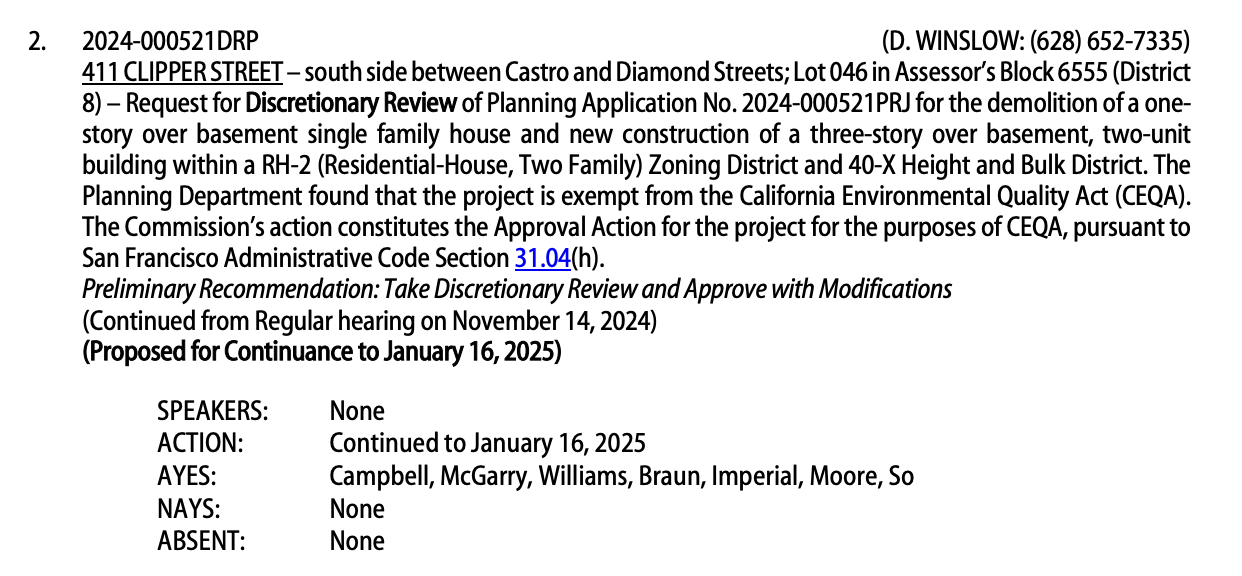
\includegraphics[width=0.8\textwidth]{sf_zoning_example_1.png}
			\label{sf_zoning_example_1}
		\end{figure}
		
		\begin{figure}[ht]
		\centering
			\caption{Example (2) of Information Contained in San Francisco Planning Commission Meeting Minutes}
			
\includegraphics[width=0.8\textwidth]{sf_zoning_example_2.png}
			\label{sf_zoning_example_2}
		\end{figure}
		
		\begin{figure}[ht]
		\centering
			\caption{Example (3) of Information Contained in San Francisco Planning Commission Meeting Minutes}
			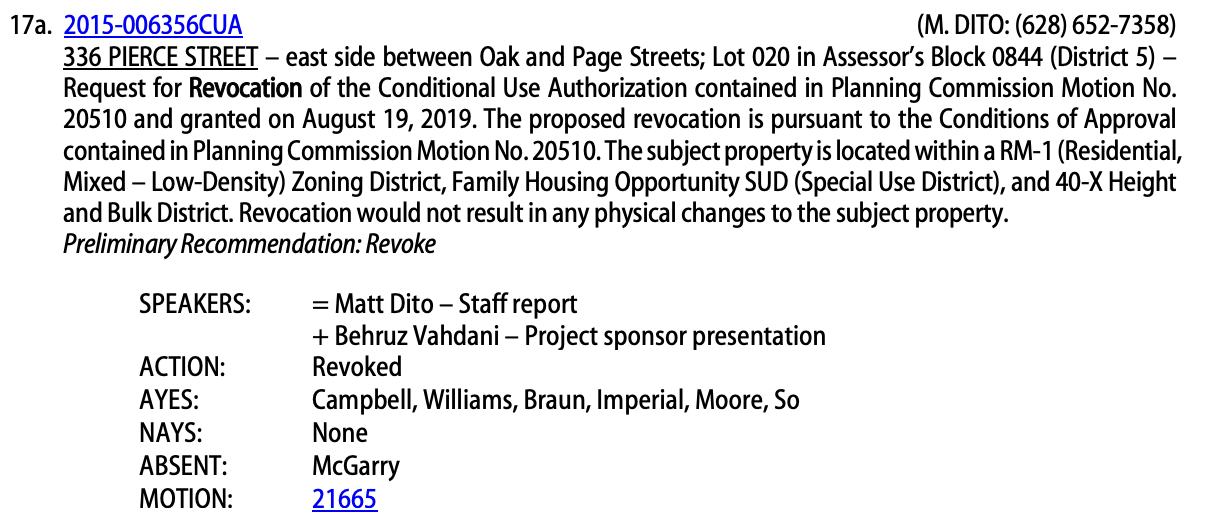
\includegraphics[width=0.8\textwidth]{sf_zoning_example_3.png}
			\label{sf_zoning_example_3}
		\end{figure}
	
\clearpage
\printbibliography

\end{document}